\section{Benchmark Integrity and Checkpoint Selection}
\label{app:data}
\subsection{Source data and split integrity}
RealRain-1k-H provides real-rain pairs; RESIDE-6K and SnowCityscapes provide
synthetic haze and snow; SmokeBench provides paired surveillance scenes~\cite{Jin_2025_SmokeBench}.
The manifest contains 22,955 active pairs and 7,115 reserves. An audit of
52,140 distinct files finds zero duplicate decoded pairs, exact cross-split
overlaps or near-target cross-split candidates under the combined rule:
pHash distance $\leq2$, aspect-ratio difference $\leq0.01$, and
$16\times16$ RGB thumbnail MAE $\leq2/255$. Within-partition near copies
share a background group. Reserves contain 5,232 snow test, 760 smoke test
and 1,123 smoke validation pairs. Incomplete sequence metadata and only six
held-out smoke backgrounds limit independence and coverage.

\subsection{Validation trajectories}
\noindent\begin{minipage}{\linewidth}
\centering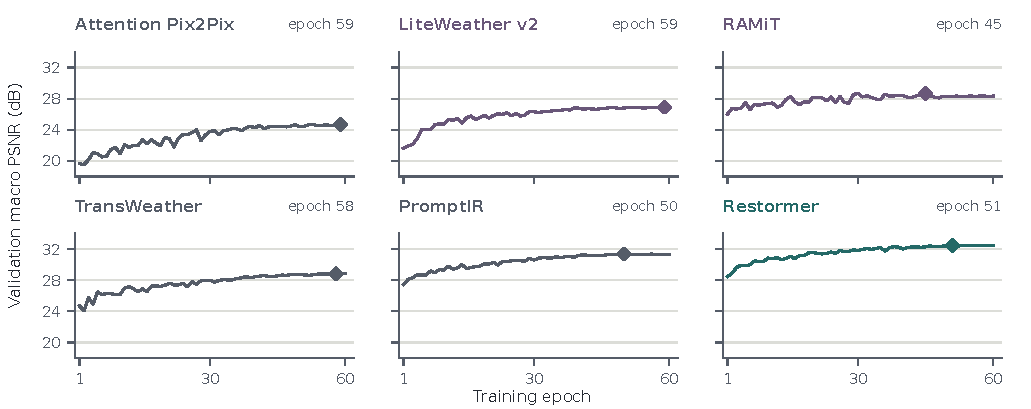
\includegraphics[width=.96\linewidth]{figures/validation_trajectories.pdf}
\captionof{figure}{Native-resolution validation PSNR across 60 epochs. Diamonds identify the best validation macro PSNR and selected epoch. Shared axes support comparison; each curve represents one training seed, with initialization sources differing across models.}
\label{fig:validation-trajectories}
\end{minipage}

Restormer selects epoch 51 at 32.45\,dB validation macro PSNR. Its compact
inference file holds 26,126,644 parameters in 104,701,712 bytes; continuation
arms start from these weights.

\subsection{Per-weather structural fidelity}
\noindent\begin{minipage}{\linewidth}
\centering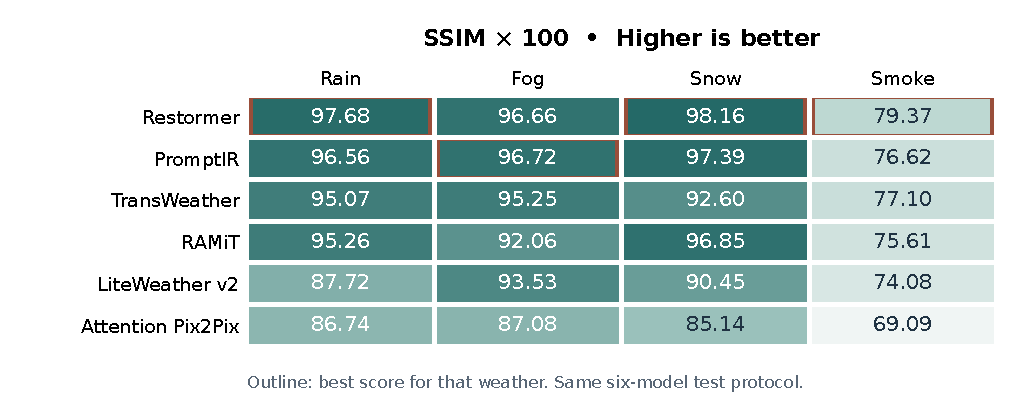
\includegraphics[width=\linewidth]{figures/weather_ssim.pdf}
\captionof{figure}{Per-weather structural similarity on 2,334 test pairs, displayed as $\mathrm{SSIM}\times100$. Outlined cells mark the best model per weather. This scaled similarity score is not detection accuracy.}
\label{fig:ssim-map}
\end{minipage}


\clearpage
\begin{multicols}{2}\raggedcolumns
The degraded-input macro is 18.62\,dB and 71.35 on the
$\mathrm{SSIM}\times100$ scale. A 2,000-resample cluster bootstrap gives
PSNR intervals of [32.00, 33.13]\,dB for Restormer and [30.81, 31.90]\,dB
for PromptIR, conditional on the trained checkpoints.

Restormer has 27 smoke PSNR regressions and 37 SSIM regressions against
raw input. Attention Pix2Pix has 179 and 341, respectively, among 342 smoke
images. The two regression sets can overlap. Display values use at most
two decimals; evidence files retain full precision.
\end{multicols}

\subsection{Preliminary rain-only baseline}
The early rain study used 784 training, 112 validation and 224 test pairs:
20 epochs, seed 42, AdamW, $128\times128$ crops and BF16 on an A100.
Validation selected epoch 15. Figure~\ref{fig:rain-progress} and
Table~\ref{tab:rain-preliminary} show mean per-image native-resolution RGB
scores for this historical checkpoint. The later four-weather benchmark
uses a distinct checkpoint and aggregation protocol.

\begin{center}\begin{minipage}{\linewidth}
\centering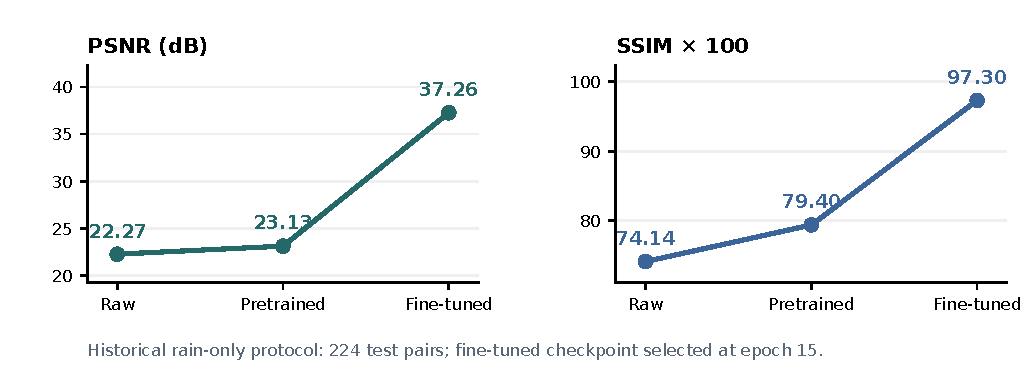
\includegraphics[width=\linewidth]{figures/historical_rain_progress.pdf}
\captionof{figure}{Measured progress in the preliminary rain-only experiment: degraded input, pretrained restoration and fine-tuned restoration. Both panels use the same 224 rain test pairs; this is separate from the six-model four-weather comparison.}
\label{fig:rain-progress}
\end{minipage}\end{center}

\begin{center}\begin{minipage}{.80\linewidth}
\centering\small
\captionof{table}{Historical rain-only benchmark; SSIM uses the $\times100$ display scale.}
\label{tab:rain-preliminary}
\begin{tabular*}{\linewidth}{@{\extracolsep{\fill}}lrr@{}}\toprule
Input or model & RGB PSNR (dB) & SSIM $\times100$\\\midrule
Raw rainy input &22.27&74.14\\
Pretrained Restormer &23.13&79.40\\
Fine-tuned Restormer, epoch 15 &37.26&97.30\\\bottomrule
\end{tabular*}
\end{minipage}\end{center}

\section{Continuation: Per-Weather Breakdown}
\label{app:joint}
The complete held-out breakdown below uses validation-selected states.
The small test differences do not change the validation replacement decision
in Section~\ref{sec:jointresults}; the epoch-51 baseline remains selected.
PSNR is in dB and SSIM is displayed on the $\times100$ scale.
\begin{center}\begin{minipage}{\linewidth}
\centering\small
\captionof{table}{Follow-up test breakdown: balanced PSNR (dB) / $\mathrm{SSIM}\times100$ for each weather. Checkpoints are selected by validation, and the original deployment model is retained before test.}
\label{tab:jointweather}
\begin{tabular}{@{}lcccc@{}}\toprule
Model / arm & Rain & Fog & Snow & Smoke\\\midrule
Original & 38.77 / 97.68 & 31.51 / 96.66 & 39.51 / 98.16 & 20.55 / 79.37\\
Continuation control & 38.70 / 97.62 & 31.79 / 96.81 & 39.57 / 98.17 & 20.75 / 79.71\\
Spatial & 38.71 / 97.63 & 31.79 / 96.82 & 39.57 / 98.17 & 20.76 / 79.71\\
Detail & 38.70 / 97.62 & 31.79 / 96.81 & 39.57 / 98.18 & 20.76 / 79.71\\
Combined & 38.70 / 97.62 & 31.80 / 96.82 & 39.57 / 98.18 & 20.76 / 79.71\\
Recipe only & 38.72 / 97.66 & 31.80 / 96.86 & 39.60 / 98.20 & 20.80 / 79.94\\
Combined + SSIM & 38.71 / 97.66 & 31.81 / 96.87 & 39.60 / 98.20 & 20.75 / 79.96\\
Combined + FFL & 38.68 / 97.59 & 31.80 / 96.82 & 39.57 / 98.17 & 20.78 / 79.66\\
Combined + recipe & 38.72 / 97.65 & 31.79 / 96.85 & 39.59 / 98.19 & 20.73 / 79.88\\
\bottomrule\end{tabular}
\end{minipage}\end{center}

\clearpage
\begingroup
\raggedbottom
\captionsetup{hypcap=false}
\section{Detection, Resolution Controls, and Nano Execution}
\label{app:hardware}

\newcommand{\AegisEvidenceColumns}[2]{%
  \noindent\begin{minipage}[t]{.477\linewidth}\vspace{0pt}#1\end{minipage}\hfill
  \begin{minipage}[t]{.477\linewidth}\vspace{0pt}#2\end{minipage}\par
}

\AegisEvidenceColumns{%
\subsection{Labelled detection protocols}
The earlier local pilot draws 72 images from 704 audited DAWN image and annotation pairs. It evaluates person, bicycle, car, motorcycle, bus, and truck. Raw, resize-only, and restored views share the same detector. Local precision and recall use each view's maximum-F1 point.

The Nano benchmark has 72 images and 541 annotations. At confidence 0.25 and IoU 0.50, unmatched predictions fall from 92 to 60 and misses rise from 271 to 431. The Nano comparison measures the complete cascade. Estimating the contribution of resampling would require a resize-only arm over the full labelled set.
}{%
\subsection{Engine identity and fixture agreement}
The original 4\,GB Nano runs L4T 32.7.3, Python 3.6.9, and TensorRT 8.2.1.8~\cite{NVIDIA_Compute,NVIDIA_TensorRT}. Its FP32 YOLOv8n passes three fixtures, with worst score error $5.51\times10^{-6}$ and box RMSE $4.63\times10^{-5}$ pixels. The epoch-51 mixed FP16/FP32 restorer passes four fixtures (Table~\ref{tab:nano-agreement}). Earlier larger builds encountered memory pressure. Section~\ref{app:quant} reports the offline export and compression screens.

\smallskip
\noindent\begin{minipage}{\linewidth}
\centering\footnotesize\renewcommand{\arraystretch}{1.12}\setlength{\tabcolsep}{3pt}
\captionof{table}{Mixed-precision $128\times128$ Nano Restormer fixture agreement. Errors use the scaled units below; $1\,\mathrm{mdB}=10^{-3}\,\mathrm{dB}$. All four fixtures pass the recorded gate.}
\label{tab:nano-agreement}
\begin{tabular}{@{}lrrr@{}}\toprule
Fixture & \shortstack{RMSE\\($\times10^{-4}$)} & \shortstack{$e_\infty$\\($\times10^{-3}$)} & \shortstack{$\Delta$PSNR\\(mdB)}\\\midrule
Fog & 1.95 & 1.72 & -1.65\\
Rain & 0.53 & 0.87 & +1.66\\
Smoke & 1.79 & 0.81 & +4.76\\
Snow & 1.35 & 1.22 & +0.09\\
\bottomrule\end{tabular}
\end{minipage}\par

}

\medskip
\noindent\begin{minipage}{\linewidth}
\centering\small\renewcommand{\arraystretch}{1.12}\setlength{\tabcolsep}{3.5pt}
\captionof{table}{Labelled DAWN results in percent. Local entries are raw / resize only / Restormer. Nano entries are YOLO only / Restormer + YOLO. Nano precision and recall use confidence 0.25 and IoU 0.50. Pooled AP is computed over 72 images.}
\label{tab:dawn-operating}
\begin{tabular}{@{}lrccccc@{}}\toprule
Subset & Images & Local AP$_{50:95}$ & Nano AP$_{50:95}$ & Nano AP$_{50}$ & Nano precision & Nano recall\\
\midrule
All & 72 & 29.97 / 29.25 / 32.86 & 29.59 / 14.50 & 44.32 / 23.06 & 74.59 / 64.71 & 49.91 / 20.33\\
Fog & 24 & 26.99 / 29.40 / 37.11 & 25.39 / 10.32 & 38.38 / 18.02 & 69.77 / 71.88 & 42.55 / 16.31\\
Rain & 24 & 38.87 / 37.07 / 37.21 & 38.91 / 29.24 & 58.74 / 39.22 & 71.76 / 65.52 & 47.24 / 19.10\\
Snow & 24 & 36.27 / 33.47 / 35.62 & 36.98 / 15.94 & 49.36 / 26.07 & 80.00 / 61.25 & 57.71 / 24.38\\
\bottomrule
\end{tabular}
\end{minipage}\par


\bigskip
\noindent\begin{minipage}{\linewidth}
\centering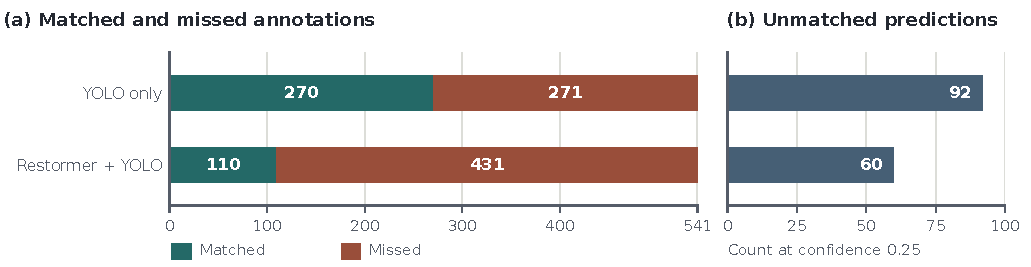
\includegraphics[width=\linewidth]{figures/nano_detection_counts.pdf}
\captionof{figure}{Object-level outcomes in labelled Nano replay. Each row in (a) accounts for all 541 annotations at confidence 0.25 and class-aware matching at IoU 0.50. The loss of matches is larger than the reduction in unmatched predictions.}
\label{fig:nano-detection-counts}
\end{minipage}

\clearpage
\subsection{Timing and power boundaries}
\AegisEvidenceColumns{%
The live application runs synthetic weather cases sequentially for about 30 seconds each. Its FPS includes capture, weather synthesis, display, and application overhead. Pipeline latency excludes weather synthesis. DAWN replay times preprocessing, transfers, inference, and NMS.
}{%
Saved-camera replay repeats 12 frames per case for at least 30 seconds. Energy integrates the board input rail, \texttt{POM\_5V\_IN}, including idle consumption. The recorded idle readings are 2.41 and 2.53\,W. These single short runs characterize the measured workloads.
}

\medskip
\noindent\begin{minipage}{\linewidth}
\centering\small\renewcommand{\arraystretch}{1.12}\setlength{\tabcolsep}{3.5pt}
\captionof{table}{Original Jetson Nano measurements. Each cell lists YOLO only / Restormer + YOLO. Live FPS includes camera and application overhead. Replay FPS excludes capture, weather synthesis, disk I/O, scoring, and output writes. Input-rail energy includes board idle consumption.}
\label{tab:nano-runtime}
\begin{tabular}{@{}llrrrr@{}}\toprule
Workload & Weather & FPS & Pipeline p50 (ms) & Input power (W) & Input J/frame\\
\midrule
Live camera & Fog & 4.72 / 0.60 & 108.2 / 1576.8 & 5.00 / 6.99 & 1.06 / 11.73\\
 & Rain & 5.02 / 0.60 & 108.4 / 1568.5 & 5.44 / 7.11 & 1.08 / 11.83\\
 & Snow & 5.28 / 0.60 & 108.4 / 1571.1 & 5.22 / 7.22 & 0.99 / 11.94\\
 & Smoke & 3.68 / 0.57 & 108.9 / 1564.8 & 4.91 / 6.91 & 1.33 / 12.21\\
\midrule
Labelled DAWN replay & Fog & 7.28 / 0.62 & 129.2 / 1596.7 & 5.71 / 7.11 & 0.78 / 11.40\\
 & Rain & 6.55 / 0.61 & 147.2 / 1617.0 & 5.38 / 7.13 & 0.82 / 11.59\\
 & Snow & 6.58 / 0.61 & 140.4 / 1619.6 & 5.34 / 6.95 & 0.81 / 11.35\\
\midrule
Saved-camera replay & Fog & 9.16 / 0.64 & 108.7 / 1560.6 & 6.17 / 7.02 & 0.67 / 10.95\\
 & Rain & 8.96 / 0.64 & 111.2 / 1562.6 & 6.11 / 7.09 & 0.68 / 11.08\\
 & Snow & 9.11 / 0.64 & 109.1 / 1556.3 & 6.18 / 7.17 & 0.68 / 11.15\\
 & Smoke & 9.11 / 0.64 & 109.1 / 1554.2 & 6.16 / 7.15 & 0.68 / 11.12\\
\bottomrule
\end{tabular}
\end{minipage}\par


\bigskip
\subsection{Saved-camera replay fidelity}
The replay compares degraded and restored frames against the same pre-mask
reference. Fog PSNR rises from 17.22 to 21.38\,dB, while SSIM falls from
90.00 to 75.67 on the $\mathrm{SSIM}\times100$ scale. Both metrics decline
in rain, snow and smoke. These pixel scores include resampling; the labelled
DAWN benchmark separately measures detection.

\begin{center}\begin{minipage}{\linewidth}
\centering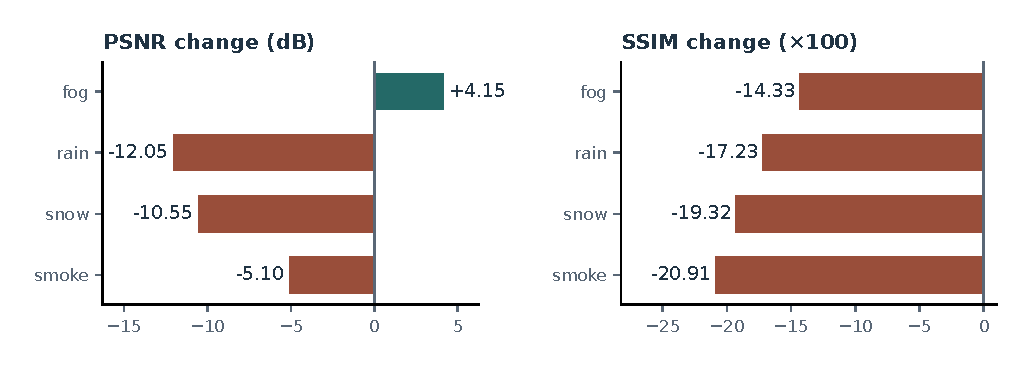
\includegraphics[width=\linewidth]{figures/camera_fidelity_scaled.pdf}
\captionof{figure}{Changes in pixel fidelity on saved-camera replay. SSIM differences use the $\times100$ display scale; neither panel measures detection accuracy.}
\label{fig:replay-fidelity}
\end{minipage}\end{center}

\clearpage
\subsection{Matched local resolution diagnostic}
\AegisEvidenceColumns{%
The diagnostic uses a $600\times315$ hazy DAWN image with two labelled vehicles, a $224\times180$ hazy RTTS photo with three labelled people, and an unlabelled $320\times240$ camera image. Fog, rain, snow, or smoke is applied once at source size (level 2, seed 43, time 0). The original views retain any pre-existing haze.

The 128 and 256 canvases preserve aspect ratio and use edge padding. Native Restormer pads to a multiple of eight and crops back. All paths return to source geometry before a $640\times640$ detector letterbox.
}{%
Six views share each degraded source, yielding 90 verified paths. Restoration uses CPU FP32. The same FP32 ONNX detector uses confidence 0.25, NMS IoU 0.7, and class-aware matching at IoU 0.50.

Across the eight added-weather variants of the labelled scenes, direct detection yields 19/0/1 (TP/FP/FN). The 256 resize-only and restored paths yield 20/2/0 and 19/4/1, respectively. Native restoration yields 19/1/1. It retains all three people under added weather and introduces one unmatched rain prediction. The same five annotations recur across conditions.
}

\medskip
\noindent\begin{minipage}{\linewidth}
\centering\small\renewcommand{\arraystretch}{1.12}\setlength{\tabcolsep}{3.5pt}
\captionof{table}{Controlled local FP32 diagnostic. Weather is applied at source resolution before branching. Labelled rows report TP/FP/FN at confidence 0.25 and IoU 0.50. Camera rows count predictions. Each source is reused across conditions.}
\label{tab:resolution-control}
\begin{tabular}{@{}lrrrrrr@{}}\toprule
Weather & Direct & 128 resize & 128 restore & 256 resize & 256 restore & Native restore\\
\midrule
\multicolumn{7}{@{}l}{\textbf{Truck/car scene, 2 labelled vehicles}}\\
Original & 2/0/0 & 1/0/1 & 1/0/1 & 2/0/0 & 2/0/0 & 2/0/0\\
Fog & 2/0/0 & 1/0/1 & 1/0/1 & 2/0/0 & 2/0/0 & 2/0/0\\
Rain & 1/0/1 & 1/1/1 & 1/0/1 & 2/0/0 & 2/0/0 & 2/0/0\\
Snow & 2/0/0 & 1/0/1 & 2/0/0 & 2/1/0 & 2/1/0 & 2/0/0\\
Smoke & 2/0/0 & 1/0/1 & 1/0/1 & 2/0/0 & 2/0/0 & 1/0/1\\
\midrule
\multicolumn{7}{@{}l}{\textbf{Small-source scene, 3 labelled people}}\\
Original & 3/0/0 & 3/0/0 & 3/0/0 & 3/0/0 & 3/1/0 & 3/1/0\\
Fog & 3/0/0 & 2/0/1 & 3/0/0 & 3/1/0 & 3/1/0 & 3/0/0\\
Rain & 3/0/0 & 3/0/0 & 3/0/0 & 3/0/0 & 3/0/0 & 3/1/0\\
Snow & 3/0/0 & 2/0/1 & 2/0/1 & 3/0/0 & 2/1/1 & 3/0/0\\
Smoke & 3/0/0 & 3/1/0 & 3/0/0 & 3/0/0 & 3/1/0 & 3/0/0\\
\midrule
\multicolumn{7}{@{}l}{\textbf{Unlabelled camera frame, prediction counts}}\\
Original & 2 & 3 & 3 & 2 & 2 & 2\\
Fog & 2 & 2 & 2 & 2 & 2 & 2\\
Rain & 2 & 3 & 3 & 2 & 2 & 2\\
Snow & 2 & 3 & 3 & 3 & 3 & 2\\
Smoke & 2 & 3 & 3 & 2 & 2 & 2\\
\bottomrule
\end{tabular}
\end{minipage}\par

\medskip

\noindent\begin{minipage}{\linewidth}
\centering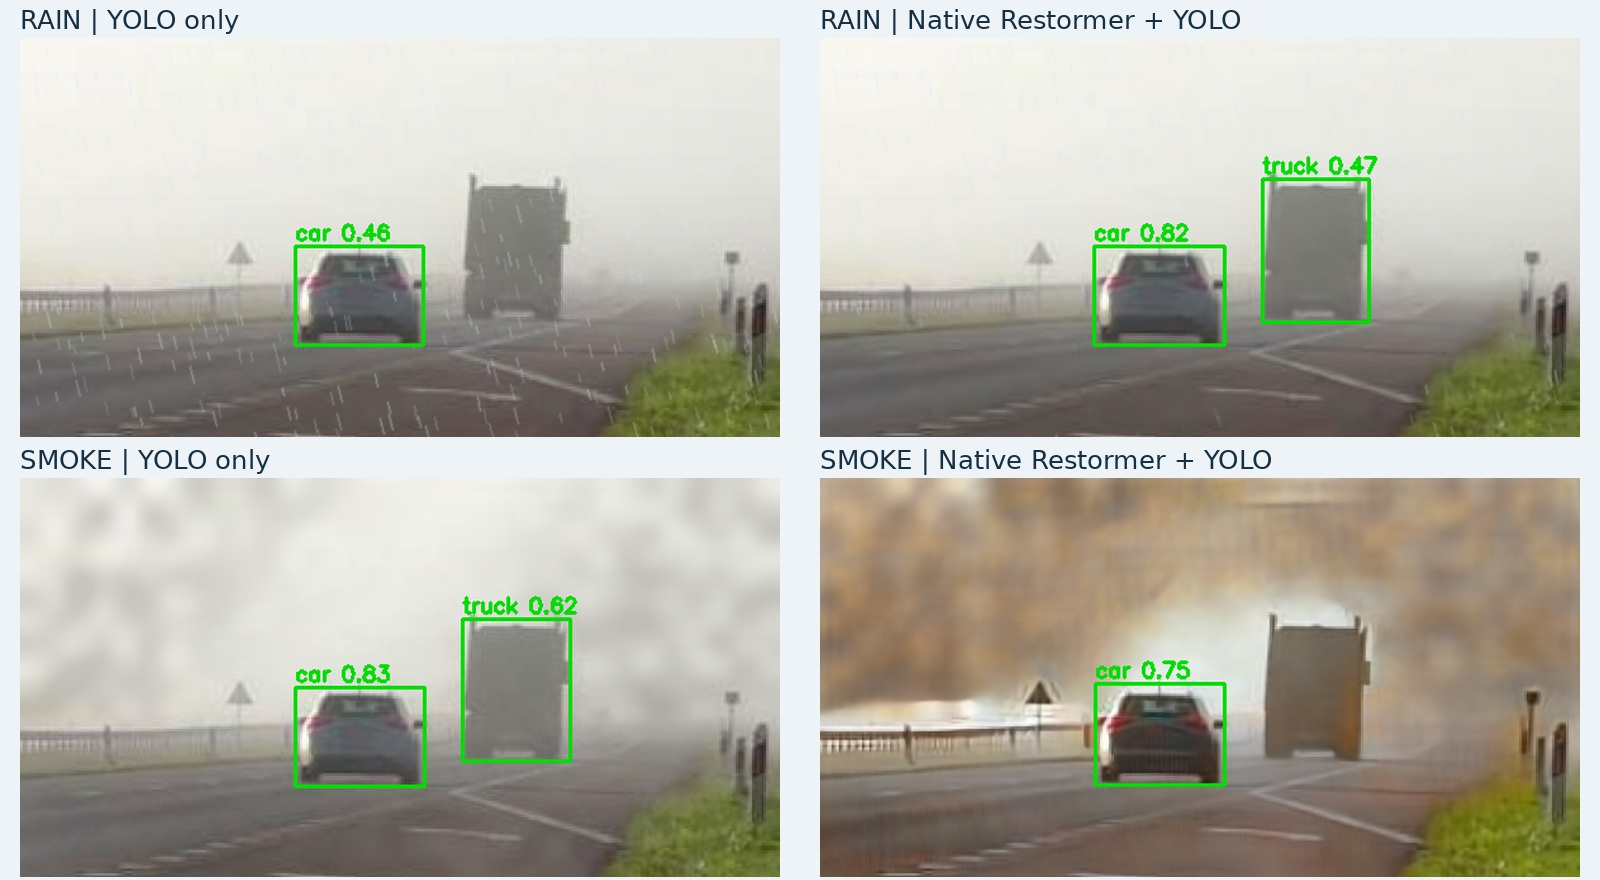
\includegraphics[width=.88\linewidth]{figures/native_detection_cases.jpg}
\captionof{figure}{Fixed-input native-resolution comparisons for the DAWN truck/car scene. The same detector finds the truck after restoration under rain and misses it after restoration under smoke. The overlays illustrate the matched counts in Table~\ref{tab:resolution-control}.}
\label{fig:native-truck}
\end{minipage}

\clearpage
\subsection{Fixed-canvas and camera controls}
\AegisEvidenceColumns{%
In the earlier fixed-$128\times128$ controls, weather is added after resizing. The people and vehicle images retain $128\times103$ and $128\times67$ pixels before padding. The truck is about $18\times26$ pixels after resizing. Resize alone removes its match in the hazy original. The small-source original retains all three people across paths.
}{%
The camera delivers $320\times240$ directly. The first of three captured frames occupies $128\times96$ before padding. Native local views yield two predictions per condition with or without restoration. The camera views lack ground-truth annotations.
}

\medskip
\noindent\begin{minipage}{\linewidth}
\centering
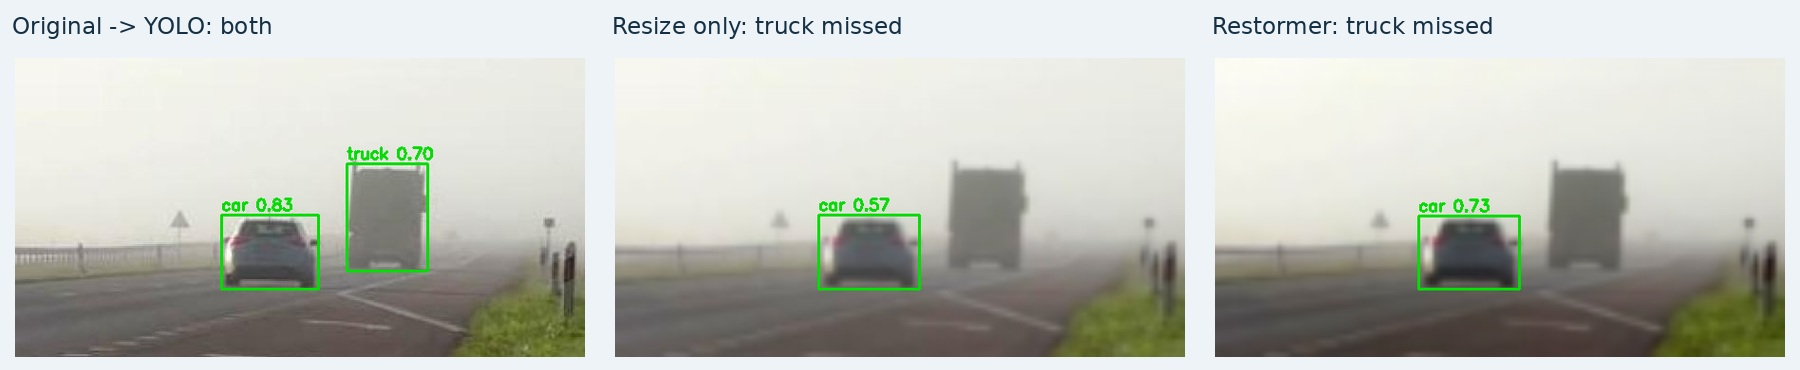
\includegraphics[width=.84\linewidth]{figures/truck_128_control.jpg}\par\smallskip
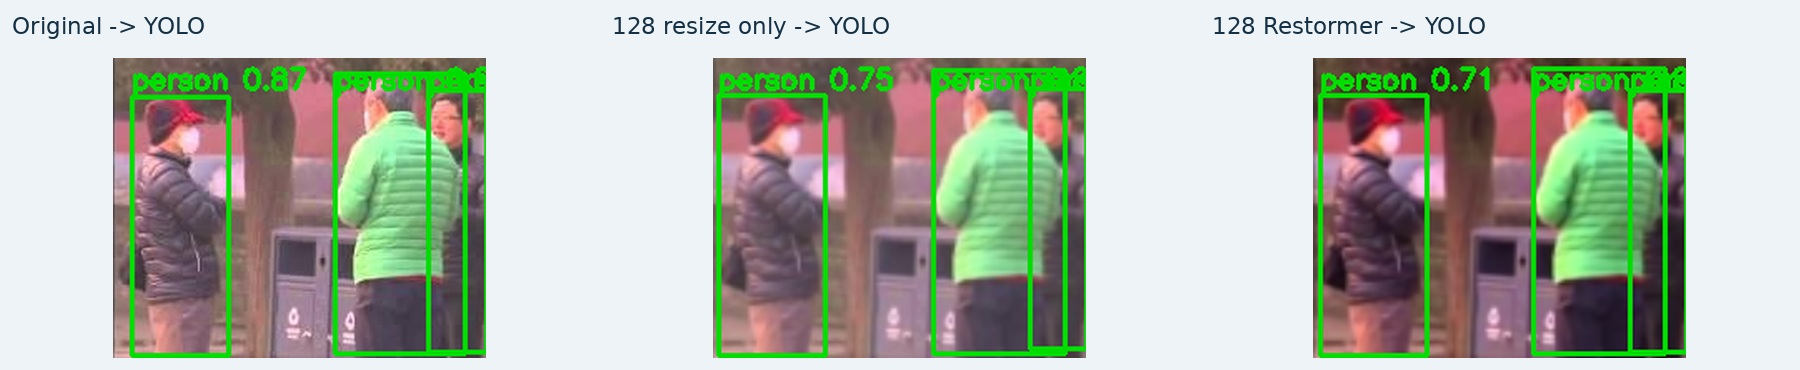
\includegraphics[width=.84\linewidth]{figures/small_source_128_control.jpg}
\captionof{figure}{Fixed-canvas controls without added synthetic weather. The truck is detected at source size and missed in both 128 paths. All three paths detect the annotated people in the small RTTS source. Images are enlarged from saved outputs.}
\label{fig:fixed-canvas}
\end{minipage}

\medskip
\noindent\begin{minipage}{\linewidth}
\centering\small\renewcommand{\arraystretch}{1.12}\setlength{\tabcolsep}{3.5pt}
\captionof{table}{Fixed-$128\times128$ Nano diagnostics. Synthetic weather is added after resizing. Labelled rows show TP/FP/FN. Camera entries count predictions. Timing is median pipeline latency over repeated calls on each input.}
\label{tab:fixed-diagnostics}
\begin{tabular}{@{}llrrr@{}}\toprule
Source & Weather & Resize + YOLO & Restormer + YOLO & Median ms, resize / restored\\
\midrule
RTTS people & Original & 3/0/0 & 3/0/0 & 117.1 / 1554.7\\
 & Rain & 2/0/1 & 2/1/1 & 115.7 / 1560.3\\
 & Snow & 2/0/1 & 2/0/1 & 114.5 / 1560.6\\
 & Smoke & 3/1/0 & 3/0/0 & 116.9 / 1561.8\\
\midrule
DAWN truck/car & Original & 1/0/1 & 1/0/1 & 119.1 / 1563.6\\
 & Rain & 0/1/2 & 1/0/1 & 120.3 / 1562.7\\
 & Snow & 1/0/1 & 1/0/1 & 122.4 / 1566.8\\
 & Smoke & 1/0/1 & 1/0/1 & 120.5 / 1566.8\\
\midrule
320 × 240 camera & Original & 3 & 3 & 115.4 / 1564.7\\
 & Rain & 4 & 2 & 118.7 / 1563.0\\
 & Snow & 4 & 4 & 119.0 / 1562.2\\
 & Smoke & 3 & 2 & 116.8 / 1565.0\\
\bottomrule
\end{tabular}
\end{minipage}\par


\medskip
\noindent\begin{minipage}{\linewidth}
\centering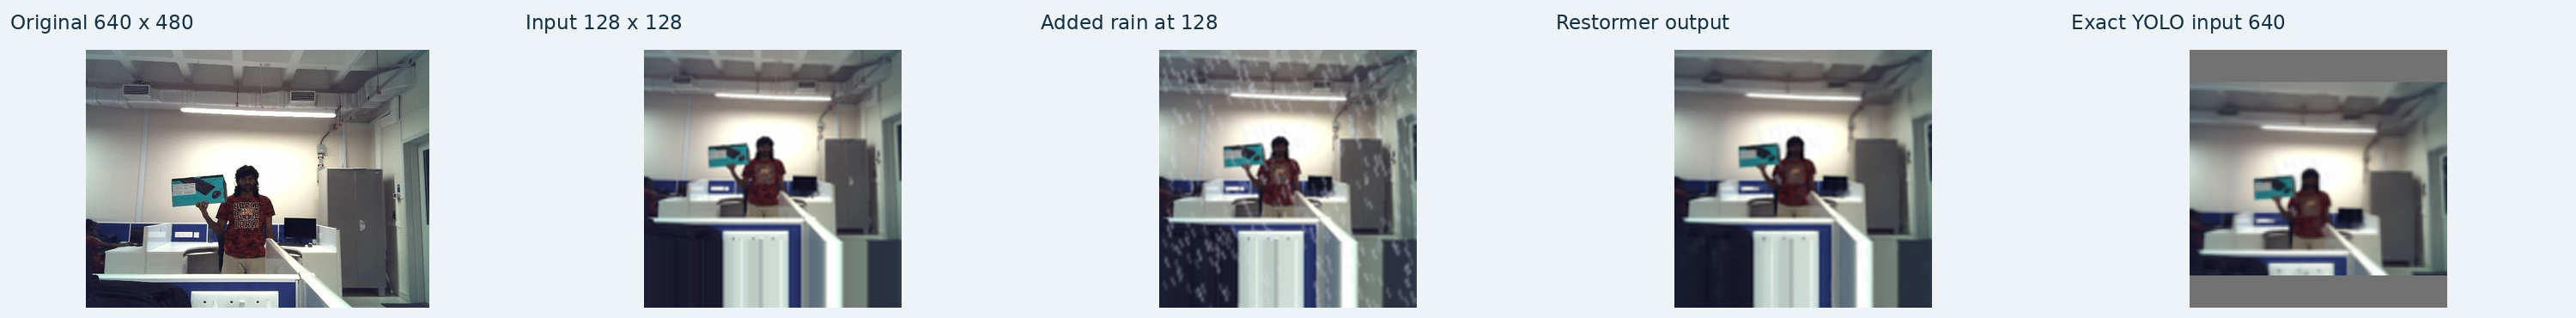
\includegraphics[width=.94\linewidth]{figures/camera_path_example.jpg}
\captionof{figure}{A separate saved $640\times480$ camera frame. The frame occupies $128\times96$ image pixels before padding. Synthetic rain is applied on the canvas. The restored result maps back to source geometry for detection.}
\label{fig:camera-path}
\end{minipage}
\clearpage
\endgroup

\clearpage
\section{Reproducibility and Evidence Map}
\label{app:repro}
\subsection{Records needed to reproduce the report}
The report uses saved experiment outputs; its preparation did not retrain
models, rerun full-set inference, or repeat board measurements. The manuscript
evidence verifier checks 35 file hashes, split counts and groups, six-model
native test aggregates, checkpoint identities, continuation results and the
local detection table. The later Nano source index supplies separate hashes
for the November 11 summaries and resolution controls.

\begin{table}[htbp]
\centering\small
\caption{Repository evidence map. Paths are relative to the project root.
The accompanying report audit records input hashes and figure/table use.}
\label{tab:evidence-map}
\begin{tabularx}{\textwidth}{@{}p{.22\textwidth}Y@{}}
\toprule Report component & Primary records and implementation\\\midrule
Frozen paired split & \path{data/manifests/weather_v3/active.csv}; \path{docs/manuscript/evidence/data_protocol.json}; \path{src/aegis_perception/data/sampling.py}\\
Model identity and quality & \path{docs/manuscript/evidence/six_models.json}; \path{docs/manuscript/tables/six_models.csv}; \path{artifacts/models/index.json}\\
Aggregation and uncertainty & \path{src/aegis_perception/evaluation.py}; \path{docs/manuscript/evidence/per_image_restoration.csv.gz}\\
Restorer implementation & \path{src/aegis_perception/models/restormer.py}; \path{src/aegis_perception/models/liteweatherformer_v2.py}; \path{configs/restoration/official_v1/sources.json}\\
Continuation and calibration & \path{docs/manuscript/evidence/joint_experiments.json}; \path{configs/restoration/joint_v3/}; \path{research/restormer_joint_v3/}\\
Local DAWN pilot & \path{docs/manuscript/tables/detection_pilot72.csv}; \path{scripts/deployment/edge_dawn.py}\\
Compression screens & \path{docs/manuscript/evidence/custom_quantization_screen.json}; \path{docs/manuscript/tables/pruning_screen.csv}\\
Nano accuracy and runtime & \path{artifacts/edge_v1/nano_20261111/consolidated_report_v2/sources/}; \path{scripts/weather_testing/score_nano_real.py}\\
Matched resolution & \path{artifacts/edge_v1/nano_20261111/resolution_accuracy_v1/}; source and detector-input verification for 90 paths\\
\bottomrule
\end{tabularx}
\end{table}

\subsection{Checkpoint and metric identity}
The selected six-model Restormer is epoch 51. Its compact inference file has
SHA-256
\begin{quote}\small\ttfamily
5268af32c161413502a8978a839b3111\\
52a1dd2bf093ade137e07d58166a8555
\end{quote}
The original deraining initialization, historical epoch-15 rain model,
earlier four-weather run and continuation arms must not be substituted for
this checkpoint. The same rule applies to model version: the evaluated
LiteWeather v2 is not the retained legacy convolutional implementation.

Image-based PSNR and SSIM use clean targets. Export agreement compares two
model outputs. AP uses labelled objects and explicitly configured confidence,
matching and suppression rules. Runtime uses the timing boundary of its
workload. These measures answer different questions even when they share
an input image or checkpoint.

\subsection{Interpretation of dated evidence}
The 5 November deployment notes describe a period before the later complete
Nano measurements. The 11 November accuracy and telemetry records establish
that the stated replay and live workloads ran; they do not establish sustained
operational acceptance. Historical documents are preserved with their original
status. Present-day report statements use the relevant dated record instead
of merging planned Orin performance with measured original-Nano performance.

\subsection{Result precision and reuse}
Numerical tables and charts use at most two decimals for readability. Small
agreement errors are displayed in scaled units, and SSIM is shown as
$\mathrm{SSIM}\times100$ where labelled. Rounding affects presentation only;
checkpoint selection and acceptance decisions use the saved full-precision
records. Independent reproduction of the experiments requires the original
data, weights, configurations and target hardware.
